\chapter{Sound Waves in Fluids}\label{ch:b2:sound-waves}

Count the seconds between the flash and the thunder and divide by
three: that is the distance in kilometres. Sound crosses air at a
third of a kilometre per second, water at a kilometre and a half, and
an ultrasound scanner times the echoes from inside the body to a
millionth of a second to draw its picture. This chapter applies the
fluid mechanics of \cref{ch:b2:euler-bernoulli,ch:b2:fluid-kinematics}
to a fluid at rest disturbed by a small pressure ripple, and finds the
\omterm{thm:b2:waves-on-strings:equation}{d'Alembert equation} again: the \omterm{thm:b2:sound-waves:equation}{speed of sound}, what carries the
energy, how loud is loud, how sound spreads in space, and why a siren
changes pitch as it passes.

\section{The acoustic approximation}

\begin{definition}[Acoustic perturbation]\label{def:b2:sound-waves:approximation}
\index{acoustic approximation}\index{overpressure}
A fluid at rest, of uniform pressure $P_0$ and density $\rho_0$, is
disturbed: $P = P_0 + p(M, t)$, $\rho = \rho_0 + \rho_1(M, t)$, velocity
$\vect v(M, t)$. The \emph{acoustic approximation} keeps only the first
order in the small quantities $p$ (the \emph{overpressure}, or acoustic
pressure), $\rho_1$ and $\vect v$: $|p| \ll P_0$, $|\rho_1| \ll \rho_0$, $v \ll c$,
and the transformation undergone by each \omterm{def:b2:fluid-kinematics:particle}{fluid particle} is so fast
that it exchanges no heat: it is \emph{isentropic}, with the
compressibility $\chi_S = \frac1\rho\bigl(\frac{\partial\rho}{\partial P}\bigr)_S$.
Gravity is neglected.
\end{definition}

\begin{theorem}[Sound waves]\label{thm:b2:sound-waves:equation}
\index{speed of sound}\index{wave equation (acoustics)}
To first order, \omterm{thm:b2:euler-bernoulli:euler}{Euler's equation}, mass conservation and the isentropic
law read
\[
\rho_0\frac{\partial\vect v}{\partial t} = -\operatorname{\vect{grad}}p , \qquad
\frac{\partial\rho_1}{\partial t} + \rho_0\operatorname{div}\vect v = 0 , \qquad
\rho_1 = \rho_0\chi_Sp ,
\]
and together they give the \omterm{thm:b2:waves-on-strings:equation}{wave equation} for the \omterm{def:b2:sound-waves:approximation}{overpressure},
\[
\Delta p = \frac1{c^2}\frac{\partial^2p}{\partial t^2} , \qquad
c = \frac1{\sqrt{\rho_0\chi_S}} ,
\]
(the same for $\rho_1$ and for $\vect v$). For a perfect gas, $\chi_S =
1/\gamma P_0$ and
\[
c = \sqrt{\frac{\gamma P_0}{\rho_0}} = \sqrt{\frac{\gamma RT}{M}} :
\]
\qty{343}{m/s} in air at \qty{20}{\degreeCelsius}, rising by \qty{0.6}{m/s}
per kelvin; \qty{1000}{m/s} in helium; \qty{1480}{m/s} in water ($\chi_S =
\qty{4.5e-10}{Pa^{-1}}$).
\end{theorem}

\begin{proof}
Euler: the convective term $\rho(\vect v\cdot\operatorname{\vect{grad}})\vect v$
is second order, $\rho\,\partial_t\vect v \approx \rho_0\,\partial_t\vect v$, and
$\operatorname{\vect{grad}}P = \operatorname{\vect{grad}}p$. Mass: $\partial_t\rho +
\operatorname{div}(\rho\vect v) \approx \partial_t\rho_1 + \rho_0\operatorname{div}\vect v$.
Isentropic law: $\dd\rho = \rho\chi_S\,\dd P$ to first order. Take the
divergence of the first equation and the time derivative of the second:
$\rho_0\partial_t\operatorname{div}\vect v = -\Delta p = -\partial_t^2\rho_1 = -\rho_0\chi_S
\partial_t^2p$. For the perfect gas, $PV^\gamma$ constant along an isentropic
transformation gives $\dd\rho/\rho = \dd P/\gamma P$, hence $\chi_S = 1/\gamma P$,
and $P_0/\rho_0 = RT/M$.
\end{proof}

\begin{remark}[Why isentropic]\label{rem:b2:sound-waves:laplace}
Newton computed the \omterm{thm:b2:sound-waves:equation}{speed of sound} with the isothermal compressibility,
$\sqrt{P_0/\rho_0} = \qty{290}{m/s}$, $15\%$ too low; Laplace saw that the
compressions are too fast for heat to flow between the warm crests and
the cool troughs --- over one period, heat diffuses a few micrometres
(\cref{ch:b2:heat-conduction}), nothing compared with a wavelength ---
so the transformation is adiabatic and reversible, and $\gamma$ appears.
The \omterm{thm:b2:sound-waves:equation}{speed of sound} is thus a direct measurement of $\gamma$: $1.40$ for
air, $1.67$ for argon.
\end{remark}

\begin{omfigure}
\begin{tikzpicture}[font=\small, x=1cm, y=1cm, >=Stealth]
  \begin{scope}
    \draw[thick] (-3.2,-0.8) rectangle (3.2,0.8);
    \fill[omDef!25] (-0.6,-0.8) rectangle (0.6,0.8);
    \fill[omDef!8] (-0.35,-0.8) rectangle (0.95,0.8);
    \draw[omDef, dashed] (-0.35,-0.8) -- (-0.35,0.8) (0.95,-0.8) -- (0.95,0.8);
    \draw[omThm, very thick, ->] (-1.6,0) -- (-0.65,0) node[above, font=\footnotesize, pos=0.3] {$P(x)S$};
    \draw[omThm, very thick, ->] (1.6,0) -- (0.65,0) node[above, font=\footnotesize, pos=0.3] {$P(x+\dd x)S$};
    \node[font=\footnotesize] at (-0.6,-1.1) {$x$}; \node[font=\footnotesize] at (0.65,-1.1) {$x + \dd x$};
    \draw[omDef, ->] (-0.6,1.05) -- (-0.35,1.05) node[above, font=\footnotesize, pos=1.4] {$\xi(x)$};
    \node[font=\footnotesize] at (0,-1.7) {$\rho_0\,\partial_t v = -\partial_x p$, \quad $\rho_1 = -\rho_0\,\partial_x\xi = \rho_0\chi_S\,p$};
  \end{scope}
  \begin{scope}[xshift=8.2cm]
    \foreach \x in {-2.6,-2.45,...,2.6} {
      \pgfmathsetmacro{\d}{0.18*sin(deg(2.4*\x))}
      \draw[omDef, thick] ({\x+\d},-0.8) -- ({\x+\d},0.8);
    }
    \node[font=\scriptsize] at (-1.6,-1.1) {compression}; \node[font=\scriptsize] at (0,-1.1) {rarefaction}; \node[font=\scriptsize] at (1.6,-1.1) {compression};
    \draw[omThm, thick, ->] (-0.4,1.1) -- (0.8,1.1) node[right, font=\footnotesize] {$c$};
    \node[font=\footnotesize] at (0,-1.7) {a plane sound wave: the fluid slabs crowd and spread};
  \end{scope}
\end{tikzpicture}

{\small Left: a slab of fluid displaced by $\xi(x, t)$ and pushed by
the pressures on its faces; its compression sets the \omterm{def:b2:sound-waves:approximation}{overpressure}.
Right: a plane sound wave --- alternate zones of compression and
rarefaction moving at $c$, the fluid itself oscillating back and forth
along the direction of propagation (a \omterm{prop:b2:waves-on-strings:chain}{longitudinal wave}).}
\end{omfigure}

\section{Plane waves, impedance, intensity}

\begin{proposition}[Plane progressive sound wave]\label{prop:b2:sound-waves:plane}
\index{acoustic impedance}\index{acoustic intensity}\index{energy density (acoustic)}
For a plane wave $p = f(x - ct)$ travelling toward $+x$, the fluid
velocity is along $x$, in phase with the \omterm{def:b2:sound-waves:approximation}{overpressure}, and
\[
p = Z\,v , \qquad Z = \rho_0c = \sqrt{\rho_0/\chi_S} ,
\]
where $Z$ is the \emph{\omterm{prop:b2:sound-waves:plane}{acoustic impedance}} of the medium
(\unit{kg.m^{-2}.s^{-1}}): \qty{410}{kg.m^{-2}.s^{-1}} for air, \qty{1.5e6}{kg.m^{-2}.s^{-1}}
for water, $\sim\qty{1.6e6}{kg.m^{-2}.s^{-1}}$ for soft tissue,
\qty{4e7}{kg.m^{-2}.s^{-1}} for steel. The wave carries the energy density and
the intensity (power per unit area, toward $+x$)
\[
e = \tfrac12\rho_0v^2 + \tfrac12\chi_Sp^2 , \qquad I = p\,v ,
\]
which obey $\partial_te + \partial_xI = 0$; for the progressive wave the two
halves of $e$ are equal and $I = p^2/Z = Zv^2$. A sinusoidal wave of
pressure amplitude $p_m$ has the mean intensity $\langle I\rangle = p_m^2/2Z$.
\end{proposition}

\begin{proof}
For $p = f(x - ct)$, $\rho_0\partial_tv = -\partial_xp = f'/c\cdot c\dots$: precisely,
$\rho_0\partial_tv = -f'(x - ct)$, and $v = f(x - ct)/\rho_0c$ satisfies it. The
potential term of $e$ is the work stored in compressing the fluid
(an isentropic compression of unit volume by $\dd V/V = -\chi_S\,\dd p$
stores $\int p\,\chi_S\dd p = \tfrac12\chi_Sp^2$); $I$ is the work rate of the
pressure force $pS$ on the fluid ahead, moving at $v$, per unit area.
Balance: $\partial_te = \rho_0v\partial_tv + \chi_Sp\partial_tp = -v\partial_xp - p\partial_xv =
-\partial_x(pv)$ by the two linearized equations.
\end{proof}

\begin{definition}[Sound level]\label{def:b2:sound-waves:decibel}
\index{decibel}\index{sound level}\index{hearing threshold}
The \emph{sound level} of a wave of mean intensity $I$ is
\[
L = 10\log_{10}\frac I{I_0} \ \text{dB} , \qquad I_0 = \qty{1e-12}{W/m^2}
\]
--- the threshold of hearing at \qty{1}{kHz}, corresponding in air to the
pressure amplitude $p_0 \approx \qty{2e-5}{Pa}$ (rms) $= 2 \times 10^{-10}$
atmospheres. Doubling the intensity adds \qty{3}{dB}; ten times, \qty{10}{dB};
a hundred times the pressure amplitude, \qty{40}{dB}. Quiet room
\qty{30}{dB}, conversation \qty{60}{dB}, busy street \qty{80}{dB}, rock concert
\qty{110}{dB}, pain \qty{120}{dB} ($I = \qty{1}{W/m^2}$, $p_m = \qty{29}{Pa}$).
\end{definition}

\begin{example}[How small a sound is]\label{ex:b2:sound-waves:small}
At the threshold, \qty{1}{kHz}: $p_m = \qty{2.8e-5}{Pa}$, $v_m = p_m/Z =
\qty{7e-8}{m/s}$, and the displacement amplitude $\xi_m = v_m/\omega =
\qty{1e-11}{m}$ --- a tenth of an atomic diameter: the eardrum detects
motions smaller than an atom. At \qty{120}{dB}, $\xi_m = \qty{11}{\micro m}$,
still invisible, and $p_m/P_0 = 3 \times 10^{-4}$: even the loudest sounds
are tiny perturbations, which is why the linear theory works so well.
\end{example}

\begin{omfigure}
\begin{tikzpicture}
\begin{axis}[omaxis, axis x line=middle, axis y line=left, width=7.4cm, height=4.2cm,
    xlabel={$x$}, ylabel={}, xmin=0, xmax=6.6, ymin=-1.3, ymax=1.4, xtick=\empty, ytick=\empty, samples=100,
    xlabel style={at={(axis description cs:1.0,0.5)}, anchor=west},
    legend style={font=\scriptsize, at={(0.5,1.02)}, anchor=south, legend columns=3, draw=none, fill=none}]
  \addplot[omThm, thick, domain=0:6.28] {sin(deg(x))};
  \addplot[omDef, thick, dashed, domain=0:6.28] {sin(deg(x))};
  \addplot[omProp, thick, domain=0:6.28] {cos(deg(x))};
  \legend{$p$, $v = p/Z$, $\xi$}
\end{axis}
\end{tikzpicture}
\hfill
\begin{tikzpicture}[font=\small, x=1cm, y=1cm, >=Stealth]
  \draw[thick, ->] (0,0) -- (0,4.4);
  \foreach \l/\t in {0/threshold of hearing, 1/rustling leaves, 2/quiet room, 3/conversation, 4/busy street, 5/lorry at \qty{10}{m}, 6/rock concert, 7/pain} {
    \pgfmathsetmacro{\y}{0.6*\l}
    \draw (-0.1,\y) -- (0.1,\y);
    \node[anchor=east, font=\scriptsize] at (-0.15,\y) {\pgfmathparse{int(20*\l)}\pgfmathresult~dB};
    \node[anchor=west, font=\scriptsize] at (0.15,\y) {\t};
  }
  \node[font=\scriptsize, anchor=south] at (0,4.45) {$I$ ($\times 100$ per step)};
\end{tikzpicture}

{\small Left: in a plane progressive sound wave the \omterm{def:b2:sound-waves:approximation}{overpressure} and
the fluid velocity are in phase, and the displacement lags by a quarter
period. Right: the \omterm{def:b2:sound-waves:decibel}{decibel} scale --- each \qty{20}{dB} step multiplies the
intensity by a hundred and the pressure amplitude by ten.}
\end{omfigure}

\section{Spherical waves}

\begin{proposition}[Spherical waves and the inverse-square law]\label{prop:b2:sound-waves:spherical}
\index{spherical wave}\index{inverse-square law (sound)}
A small source radiating equally in all directions produces the
\omterm{prop:b2:sound-waves:spherical}{spherical wave}
\[
p(r, t) = \frac{A}{r}\,f\Bigl(t - \frac rc\Bigr) ,
\]
whose amplitude falls as $1/r$ and whose intensity falls as $1/r^2$:
for a source of acoustic power $\mathcal P$, $I = \mathcal P/4\pi r^2$, i.e.\
$-\qty{6}{dB}$ each time the distance doubles. Far from the source the
wave is locally plane, with $v = p/Z$ radial.
\end{proposition}

\begin{proof}
In spherical coordinates, for a function of $r$ alone, $\Delta p =
\frac1r\frac{\partial^2(rp)}{\partial r^2}$ (admitted; \cref{ch:b2:maxwell-equations}),
so $u = rp$ obeys the one-dimensional \omterm{thm:b2:waves-on-strings:equation}{wave equation} $\partial_r^2u = \partial_t^2u/c^2$,
whence $u = Af(t - r/c)$ for the outgoing wave. The power crossing a
sphere of radius $r$ is $4\pi r^2I$, constant if nothing is absorbed.
\end{proof}

\begin{example}[A siren, a conversation]\label{ex:b2:sound-waves:siren}
A \qty{10}{W} siren: $I = 10/4\pi r^2$, \qty{0.8}{W/m^2} at \qty{1}{m} (\qty{119}{dB},
pain), \qty{79}{dB} at \qty{100}{m}, \qty{59}{dB} at \qty{1}{km} --- still audible over
the city. A voice radiates about \qty{10}{\micro W}: \qty{60}{dB} at \qty{1}{m},
and \qty{40}{dB} at \qty{10}{m}. Air absorbs sound too (more at high
frequency, a few \omterm{def:b2:sound-waves:decibel}{decibels} per hundred metres at \qty{10}{kHz}), which is
why distant thunder rumbles low.
\end{example}

\section{The Doppler effect}

\begin{theorem}[Doppler effect]\label{thm:b2:sound-waves:doppler}
\index{Doppler effect}
A source emits at frequency $f$ and moves at speed $v_s$ along the line
joining it to an observer who moves at $v_o$, both speeds counted
positive when they approach each other; the sound travels at $c$ in the
air at rest. The observer receives the frequency
\[
f' = f\,\frac{c + v_o}{c - v_s} .
\]
A moving source crowds its wavefronts ahead of it ($\lambda' = (c - v_s)/f$)
and spreads them behind; a moving observer meets wavefronts at the
rate $(c + v_o)/\lambda$. For $v_s, v_o \ll c$ both give $\Delta f/f \approx
(v_s + v_o)/c$.
\end{theorem}

\begin{proof}
Moving source: the wavefronts emitted at $t$ and $t + 1/f$ are separated
by $c/f - v_s/f$ in the direction of motion, so the wavelength ahead is
$\lambda' = (c - v_s)/f$ and the frequency received by a fixed observer is
$c/\lambda'$. Moving observer: the wavelength is $\lambda = c/f$ but fronts pass
at the relative speed $c + v_o$. Combine.
\end{proof}

\begin{omfigure}
\begin{tikzpicture}[font=\small, x=1cm, y=1cm, >=Stealth]
  \begin{scope}
    \foreach \i in {0,1,2,3,4} {
      \pgfmathsetmacro{\r}{0.45*(5-\i)}
      \pgfmathsetmacro{\cx}{0.27*\i-0.23}
      \draw[omDef, thick] (\cx,0) circle (\r);
    }
    \fill[omThm] (1.12,0) circle (2pt);
    \draw[omThm, thick, ->] (1.12,0.15) -- (1.9,0.15) node[above, font=\footnotesize] {$v_s$};
    \node[font=\footnotesize] at (2.0,-2.45) {ahead: $\lambda' < \lambda$};
    \node[font=\footnotesize] at (-1.5,-2.45) {behind: $\lambda' > \lambda$};
    \node[font=\footnotesize] at (0.4,-3.2) {$f' = f\,\dfrac{c + v_o}{c - v_s}$};
  \end{scope}
  \begin{scope}[xshift=8.2cm]
    \foreach \i in {0,1,2,3,4} {
      \pgfmathsetmacro{\r}{0.4*(5-\i)}
      \pgfmathsetmacro{\cx}{0.6*\i-1.12}
      \draw[omDef, thick] (\cx,0) circle (\r);
    }
    \fill[omThm] (1.88,0) circle (2pt);
    \draw[omThm, thick, ->] (1.88,0.15) -- (2.7,0.15) node[above, font=\footnotesize] {$v > c$};
    \draw[omProp, thick] (1.88,0) -- (-0.36,2.0); \draw[omProp, thick] (1.88,0) -- (-0.36,-2.0);
    \draw (0.9,0) arc[start angle=180, end angle=138, radius=0.98] node[left, font=\footnotesize, xshift=-1pt] {$\theta$};
    \node[font=\footnotesize] at (0.3,-3.2) {Mach cone: $\sin\theta = c/v$};
  \end{scope}
\end{tikzpicture}

{\small Left: the wavefronts of a moving source crowd ahead and spread
behind --- higher pitch approaching, lower receding. Right: a source
faster than sound leaves its wavefronts behind; their envelope is the
\omterm{rem:b2:sound-waves:mach}{Mach cone}, heard on the ground as a boom.}
\end{omfigure}

\begin{example}[Sirens, radar guns, red cells]\label{ex:b2:sound-waves:dopplerex}
An ambulance siren at \qty{700}{Hz} passing at \qty{25}{m/s}: \qty{755}{Hz}
approaching, \qty{651}{Hz} receding --- a drop of a sixth of an octave,
the familiar "nee-naw" dip. A police radar gun measures the same
effect on a \qty{24}{GHz} radio wave reflected by a car (the wave is
shifted twice, by the car receiving and re-emitting): $\Delta f = 2fv/c =
\qty{4.8}{kHz}$ at \qty{30}{m/s}. An ultrasound probe at \qty{5}{MHz} aimed at
an artery hears the blood cells at $\Delta f = 2fv\cos\theta/c \approx \qty{1.6}{kHz}$
for \qty{0.5}{m/s} at \qty{60}{\degree}: an audible whistle whose pitch is the
blood speed. And the spectral lines of a receding galaxy are shifted
red by $\Delta\lambda/\lambda = v/c$ --- the formula holds for light at low speed,
with the relativistic correction beyond.
\end{example}

\begin{remark}[Supersonic]\label{rem:b2:sound-waves:mach}
\index{Mach cone}\index{sonic boom}
When $v_s > c$ the formula breaks down ($f' < 0$ ahead): no sound precedes
the source. The wavefronts emitted along the path have a conical
envelope of half-angle $\theta$ with $\sin\theta = c/v_s$ (the \emph{\omterm{rem:b2:sound-waves:mach}{Mach cone}});
the pressure jump carried by the cone is the \omterm{rem:b2:sound-waves:mach}{sonic boom}, which reaches
a listener on the ground only after the aircraft has passed --- at
Mach $2$ and \qty{10}{km} of altitude, $\theta = \qty{30}{\degree}$ and the boom
arrives $10\,\text{km}/\tan\theta/v_s \approx \qty{25}{s}$ after the overhead
passage. A bullet's crack and the tip of a whip are the same cone.
\end{remark}

\begin{method}[Orders of magnitude in acoustics]\label{met:b2:sound-waves:method}
Given a \omterm{def:b2:sound-waves:decibel}{sound level} $L$: $I = I_0\,10^{L/10}$; then $p_m = \sqrt{2ZI}$,
$v_m = p_m/Z$, $\xi_m = v_m/\omega$; the power of a source is $4\pi r^2I$ if it
radiates in all directions (twice less over a hard floor, which
reflects into a half-space). Going from $r_1$ to $r_2$ changes $L$ by
$20\log_{10}(r_1/r_2)$. Adding $n$ incoherent equal sources adds
$10\log_{10}n$; two coherent sources in phase at a point add \qty{6}{dB}.
\end{method}

\section{Exercises}

\begin{exercise}[$\star$]\label{exo:b2:sound-waves:1}
\omterm{thm:b2:sound-waves:equation}{Speed of sound} in air ($\gamma = 1.40$, $M = \qty{29}{g/mol}$) at
\qty{0}{\degreeCelsius}, \qty{20}{\degreeCelsius} and at \qty{-50}{\degreeCelsius}
(\qty{10}{km} altitude); in helium ($\gamma = 1.67$, $M = \qty{4}{g/mol}$) and
carbon dioxide ($\gamma = 1.30$, $M = \qty{44}{g/mol}$) at \qty{20}{\degreeCelsius}.
Why does a voice sound high-pitched after breathing helium?
\end{exercise}

\begin{exercise}[$\star$]\label{exo:b2:sound-waves:2}
A conversation at \qty{60}{dB}, \qty{500}{Hz}: intensity, pressure
amplitude, velocity amplitude and displacement amplitude in air
($Z = \qty{410}{kg.m^{-2}.s^{-1}}$). Same for \qty{120}{dB}. Level of two
people talking at once; of a hundred.
\end{exercise}

\begin{exercise}[$\star$]\label{exo:b2:sound-waves:3}
A loudspeaker radiates \qty{1.0}{W} of sound equally in all directions.
Intensity and level at \qty{1}{m}, \qty{10}{m}, \qty{100}{m}; distance at which
the level falls to \qty{60}{dB}; power needed for \qty{100}{dB} at \qty{30}{m}
(an open-air concert).
\end{exercise}

\begin{exercise}[$\star$]\label{exo:b2:sound-waves:4}
Thunder is heard \qty{4.5}{s} after the flash: distance. A ship's horn
echoes off a cliff after \qty{3.0}{s}: distance. Sonar: an echo from the
sea floor returns after \qty{2.4}{s} ($c = \qty{1500}{m/s}$): depth. A
\qty{5}{MHz} ultrasound echo returns after \qty{130}{\micro s} in tissue
(\qty{1540}{m/s}): depth.
\end{exercise}

\begin{exercise}[$\star\star$]\label{exo:b2:sound-waves:5}
A train horn at \qty{500}{Hz}; $c = \qty{340}{m/s}$. (a) Frequency heard by a
person on the platform as the train approaches at \qty{40}{m/s}, and
after it has passed. (b) The person is on a train moving toward the
horn at \qty{40}{m/s}, the horn at rest; then both moving toward each
other at \qty{40}{m/s}: compare with a relative speed of \qty{80}{m/s} and
one body at rest. (c) Frequency heard by the driver of the horn's train
from the echo off a wall ahead.
\end{exercise}

\begin{exercise}[$\star\star$]\label{exo:b2:sound-waves:6}
For a pressure amplitude of \qty{1.0}{Pa} at \qty{1}{kHz}, compute the
velocity and displacement amplitudes, the intensity and the level in
air, in water ($Z = \qty{1.5e6}{kg.m^{-2}.s^{-1}}$) and in steel
($\qty{4e7}{kg.m^{-2}.s^{-1}}$). Same pressure, very different intensities:
comment. (Underwater levels are quoted relative to \qty{1}{\micro Pa}: what
is \qty{1}{Pa} on that scale?)
\end{exercise}

\begin{exercise}[$\star\star$]\label{exo:b2:sound-waves:7}
(a) Newton's isothermal speed $\sqrt{P_0/\rho_0}$ for air at
\qty{20}{\degreeCelsius} ($\rho_0 = \qty{1.20}{kg/m^3}$) and Laplace's correction.
(b) Measured: \qty{343}{m/s} in air, \qty{323}{m/s} in argon ($M = \qty{40}{g/mol}$)
at \qty{20}{\degreeCelsius}: deduce $\gamma$ for each; interpret with the
number of degrees of freedom. (c) Estimate how far heat diffuses in
one period at \qty{1}{kHz} (thermal diffusivity of air
\qty{2e-5}{m^2/s}) and compare with the wavelength.
\end{exercise}

\begin{exercise}[$\star\star$]\label{exo:b2:sound-waves:8}
\emph{Organ pipes.} In a pipe the \omterm{def:b2:sound-waves:approximation}{overpressure} is zero at an open end
and the velocity is zero at a closed end. (a) \omterm{prop:b2:waves-on-strings:modes}{Standing waves} in a pipe
open at both ends: show the modes are $f_n = nc/2L$; in a pipe closed at
one end, $f_n = (2n - 1)c/4L$. (b) Lengths for a \qty{440}{Hz} fundamental
in each case. (c) Which harmonics does each pipe contain? (d) The real
open end sits about $0.6$ radius beyond the pipe (end correction): for
a \qty{4}{cm} pipe, the correction on $L$ and on $f$.
\end{exercise}

\begin{exercise}[$\star\star$]\label{exo:b2:sound-waves:9}
A \qty{2.0}{kW} electric siren converts $20\%$ of its power into sound
radiated into a half-space (it sits on a roof). (a) Intensity, level
and pressure amplitude at \qty{100}{m}. (b) Distance of the pain threshold
(\qty{120}{dB}); of the \qty{70}{dB} contour where it stops being alarming.
(c) Air absorption adds \qty{1}{dB} per \qty{100}{m} at its frequency:
distance of the \qty{70}{dB} contour now (solve numerically). (d) How many
such sirens cover a city of \qty{10}{km} radius?
\end{exercise}

\begin{exercise}[$\star\star\star$]\label{exo:b2:sound-waves:10}
\emph{Energy of a standing sound wave.} In a closed tube of length $L$
the \omterm{def:b2:sound-waves:approximation}{overpressure} is $p = p_m\cos(kx)\cos(\omega t)$, $k = n\pi/L$. (a) Find $v(x,
t)$ from the linearized Euler equation. (b) Kinetic and potential
energy densities; show that they oscillate in quadrature in time and
are shifted by a quarter wavelength in space. (c) Total energy in the
tube (section $S$); check it is constant. (d) Mean intensity: zero
everywhere --- and yet the energy moves: describe how.
\end{exercise}

\begin{exercise}[$\star\star\star$]\label{exo:b2:sound-waves:11}
\emph{\omterm{rem:b2:sound-waves:mach}{Sonic boom}.} An aircraft flies horizontally at $v = 1.6\,c$ at
altitude $h = \qty{12}{km}$, $c = \qty{300}{m/s}$ there. (a) Derive the Mach
angle from the envelope of the spherical wavefronts. (b) Time between
the overhead passage and the boom on the ground (neglect the variation
of $c$ with altitude). (c) Width on the ground of the strip that hears
the boom as the aircraft flies by, if the cone's trace is heard within
$\pm\qty{30}{km}$ of the track: why is supersonic flight over land
banned? (d) A rifle bullet at \qty{800}{m/s}: Mach angle; what an observer
standing \qty{10}{m} from the trajectory hears, and in what order.
\end{exercise}

\begin{exercise}[$\star\star\star$]\label{exo:b2:sound-waves:12}
\emph{Doppler ultrasound.} A probe emits at $f = \qty{5.0}{MHz}$ into tissue
($c = \qty{1540}{m/s}$); red cells move at $v$ along a vessel making the
angle $\theta$ with the beam. (a) Frequency received by a cell (moving
observer). (b) It re-emits (scatters) this frequency as a moving source:
frequency back at the probe; show $\Delta f = 2fv\cos\theta/c$ for $v \ll c$. (c)
$\Delta f$ for $v = \qty{0.50}{m/s}$, $\theta = \qty{60}{\degree}$; for $\theta = \qty{90}{\degree}$
--- what does the operator do? (d) The probe can resolve \qty{50}{Hz}:
velocity resolution. Why is the Doppler signal made audible rather than
displayed only?
\end{exercise}

\begin{omfigure}
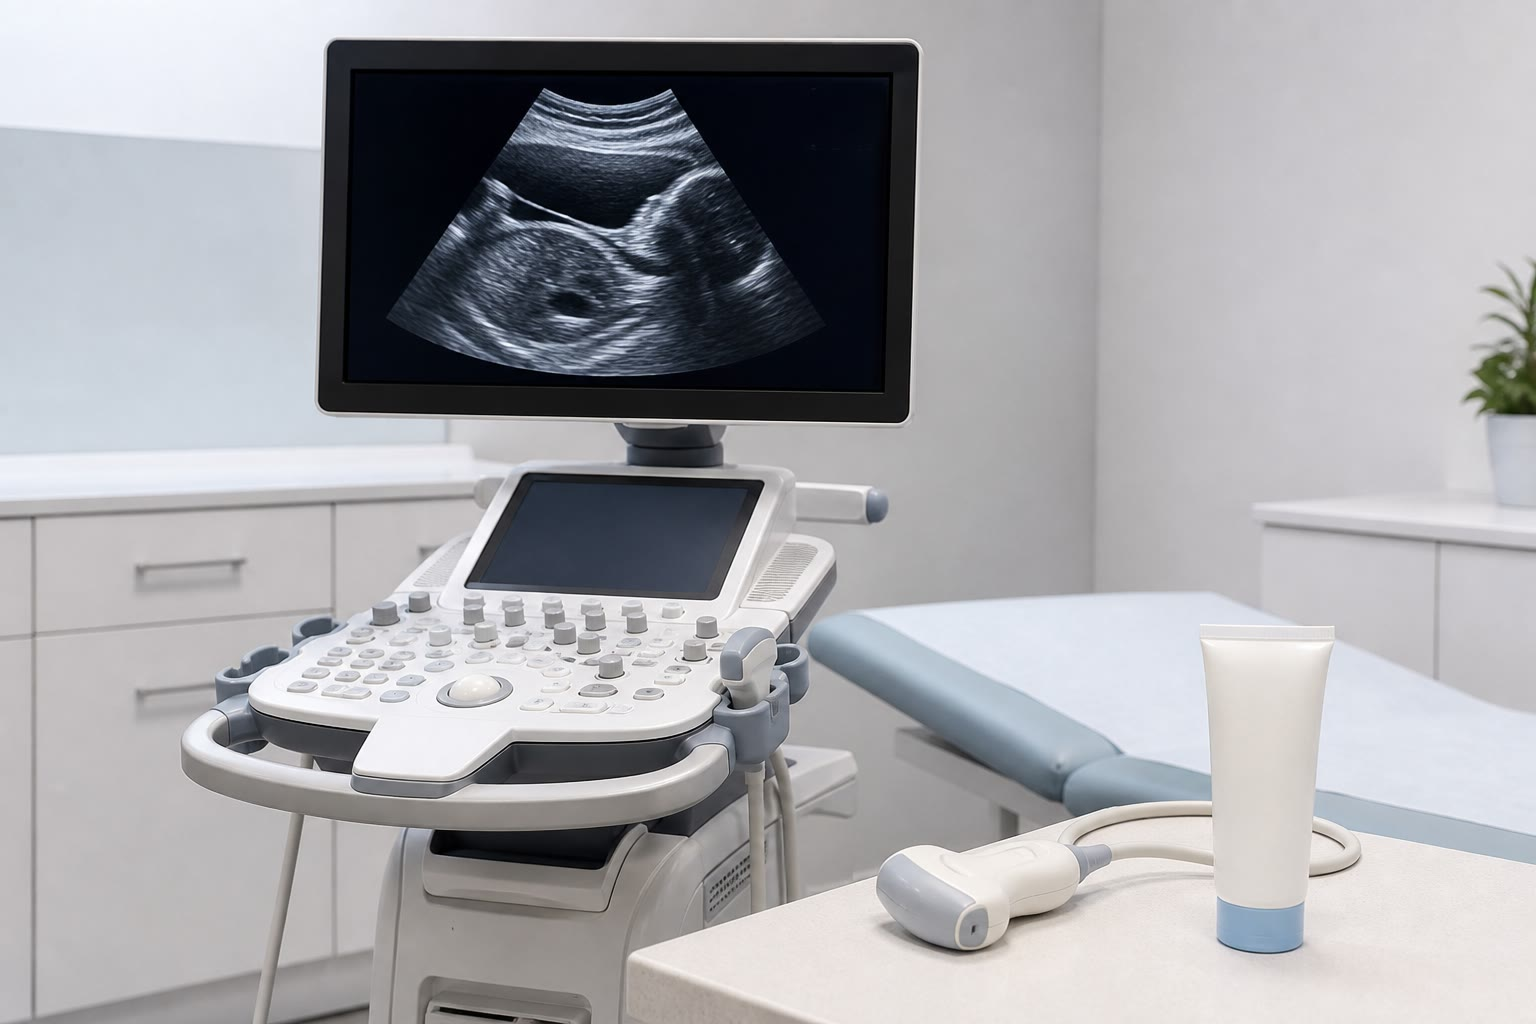
\includegraphics[width=0.58\linewidth]{images/book4/ai/b4-07-ultrasound-probe.jpg}

{\small An ultrasound scanner: a few megahertz of sound, timed echoes and the impedance mismatches between tissues draw the image; the gel removes the film of air that would reflect everything.}
\end{omfigure}

\section{Problem: From thunder to the echograph}

\begin{problem}[{Weekend problem --- sound in the open air, in a concert
hall, inside the body and from a passing siren}]
\label{pb:b2:sound-waves:1}

Air: $\gamma = 1.40$, $M = \qty{29}{g/mol}$, $Z = \qty{410}{kg.m^{-2}.s^{-1}}$ at
\qty{15}{\degreeCelsius}; $R = \qty{8.31}{J/(mol.K)}$.

\medskip
\noindent\textbf{Part I --- The storm.}
\begin{enumerate}
  \item \omterm{thm:b2:sound-waves:equation}{Speed of sound} at \qty{15}{\degreeCelsius} and at \qty{30}{\degreeCelsius};
        justify the rule "three seconds per kilometre".
  \item Thunder arrives \qty{4.0}{s} after the flash: distance of the
        strike. The thunder lasts several seconds although the flash is
        instantaneous: why?
  \item Near the strike the level reaches \qty{120}{dB}: pressure amplitude
        and velocity amplitude of the air.
  \item Energy received per square metre of wall during a thunderclap
        of \qty{2}{s} at \qty{120}{dB}.
  \item On a clear night the ground cools and the air is colder below
        than above. Sound rays obey Snell's law between layers,
        $\sin i/c = $ const: do rays launched upward bend down or up?
        Why are distant sounds heard so well at night and over water?
  \item By day, the reverse: a listener at \qty{3}{km} hears nothing.
        Estimate the angle by which a horizontal ray has bent after
        \qty{3}{km} if $c$ falls by \qty{1}{\%} per \qty{500}{m} of altitude
        (treat the bending as uniform: the ray is a circle).

  \item Air absorbs high frequencies far more than low ones: why does
        distant thunder rumble while a nearby strike cracks?
\end{enumerate}

\medskip
\noindent\textbf{Part II --- The concert.}
A loudspeaker receives \qty{100}{W} of electrical power and converts
$2\%$ of it into sound, radiated equally into the half-space in front
of it.
\begin{enumerate}[resume]
  \item Acoustic power; intensity and level at \qty{10}{m}.
  \item Pressure amplitude there; velocity and displacement amplitudes
        at \qty{100}{Hz}.
  \item Level at \qty{1}{m} (is it safe?) and distance at which the music
        falls to \qty{60}{dB}.
  \item Ten identical loudspeakers spread around the stage, not in
        phase: level at \qty{10}{m}. Two loudspeakers fed in phase, at the
        same distance from a listener on their axis: level there.
  \item The hall (volume \qty{10000}{m^3}) has \qty{2000}{m^2} of walls and audience that absorb $30\%$ of the
        sound hitting them: estimate the acoustic energy stored in the
        hall at equilibrium and the reverberation time (time for the
        level to drop \qty{60}{dB} after the music stops), using the
        balance between the power emitted and the power absorbed
        ($I_{\text{wall}} \approx ce/4$ for a diffuse field, admitted).
\end{enumerate}

\medskip
\noindent\textbf{Part III --- The echograph.}
Soft tissue: $c = \qty{1540}{m/s}$, $Z = \qty{1.6e6}{kg.m^{-2}.s^{-1}}$; bone
$Z = \qty{7e6}{kg.m^{-2}.s^{-1}}$; air $\qty{400}{kg.m^{-2}.s^{-1}}$. At normal
incidence the pressure amplitude reflected at an interface is $r = (Z_2 -
Z_1)/(Z_2 + Z_1)$ times the incident one (derived in
\cref{ch:b2:wave-interfaces}); tissue attenuates sound by about
\qty{0.5}{dB} per centimetre and per megahertz.
\begin{enumerate}[resume]
  \item Wavelength in tissue at \qty{3}{MHz}, \qty{5}{MHz}, \qty{10}{MHz}; the
        smallest detail each can resolve is about one wavelength.
  \item Echo delay from an organ \qty{12}{cm} deep; maximum rate at which
        pulses can be sent without confusing echoes; time to build an
        image of $200$ lines.
  \item Fraction of the pressure, and of the energy, reflected at a
        tissue--air interface; at a tissue--bone interface; between fat
        ($Z = \qty{1.38e6}{kg.m^{-2}.s^{-1}}$) and muscle
        ($\qty{1.70e6}{kg.m^{-2}.s^{-1}}$). Why the gel, and why bones cast
        shadows?
  \item At \qty{5}{MHz} the beam crosses \qty{2}{cm} of fat before meeting
        muscle: fraction of the emitted energy that comes back to the
        probe from that interface (reflection and round-trip
        attenuation), in \omterm{def:b2:sound-waves:decibel}{decibels}.
  \item Round-trip attenuation in \omterm{def:b2:sound-waves:decibel}{decibels} for the organ of question 12
        at each of the three frequencies; if the scanner can handle
        \qty{80}{dB} of loss, which frequencies work? State the resolution
        versus depth trade-off.
  \item The probe emits pulses of \qty{1}{\micro s} at \qty{5}{MHz}: how many
        wavelengths long is a pulse, and how does that limit the depth
        resolution?
  \item Doppler mode at \qty{5}{MHz} on an artery at \qty{0.40}{m/s}, beam at
        \qty{60}{\degree}: shift; what the operator hears.
\end{enumerate}

\medskip
\noindent\textbf{Part IV --- The siren.}
\begin{enumerate}[resume]
  \item An ambulance passes at \qty{90}{km/h} with a \qty{700}{Hz} siren:
        frequencies heard approaching and receding; the interval
        between them in semitones (a semitone is a ratio $2^{1/12}$).
  \item The listener is in a car going at \qty{15}{m/s} toward the
        approaching ambulance: frequency heard.
  \item At what instant does a listener on the pavement hear exactly
        \qty{700}{Hz}?
  \item The ambulance's wavefronts ahead of it: wavelength; speed of
        the sound relative to the ambulance ahead and behind.
  \item A radar gun at \qty{24}{GHz} reads a \qty{3.2}{kHz} shift from a car:
        speed of the car (the wave is shifted twice).
  \item Sum up: the six speeds of this problem (sound in air, in
        tissue, the ambulance, the car, the red cells, light) and the
        one formula that handles them all.
\end{enumerate}
\end{problem}
